\documentclass[11pt,a4paper]{article}

% --------------------------------
% Encoding and language
% --------------------------------
\usepackage[T1]{fontenc}
\usepackage[utf8]{inputenc}
\usepackage[english]{babel}

% --------------------------------
% Page layout
% --------------------------------
\usepackage[a4paper,margin=2.5cm]{geometry}
\usepackage{setspace}
\onehalfspacing
\usepackage{float}

% --------------------------------
% Mathematics
% --------------------------------
\usepackage{amsmath}
\usepackage{amssymb}
\usepackage{amsthm}
\usepackage{mathtools}
\usepackage{mathrsfs}

% --------------------------------
% Figures and tables
% --------------------------------
\usepackage{graphicx}
\usepackage{float}
\usepackage{caption}
\usepackage{subcaption}
\usepackage{booktabs}
\usepackage{array}
\usepackage{tikz}
\usetikzlibrary{arrows.meta,calc,patterns,positioning}

% --------------------------------
% Colors and hyperlinks
% --------------------------------
\usepackage{xcolor}
\usepackage{hyperref}
\usepackage[nameinlink,noabbrev]{cleveref}

\hypersetup{
    colorlinks=true,
    linkcolor=blue,
    citecolor=blue,
    urlcolor=blue
}

% --------------------------------
% Bibliography
% --------------------------------
\usepackage[numbers,sort&compress]{natbib}

% --------------------------------
% Lists and formatting
% --------------------------------
\usepackage{enumitem}
\usepackage{microtype}

% --------------------------------
% Theorem environments
% --------------------------------
\theoremstyle{plain}
\newtheorem{theorem}{Theorem}[section]
\newtheorem{lemma}[theorem]{Lemma}
\newtheorem{proposition}[theorem]{Proposition}
\newtheorem{corollary}[theorem]{Corollary}

\theoremstyle{definition}
\newtheorem{definition}[theorem]{Definition}
\newtheorem{example}[theorem]{Example}

\theoremstyle{remark}
\newtheorem{remark}[theorem]{Remark}

% --------------------------------
% Custom commands
% --------------------------------
\newcommand{\R}{\mathbb{R}}
\newcommand{\N}{\mathbb{N}}
\newcommand{\Z}{\mathbb{Z}}
\newcommand{\Q}{\mathbb{Q}}
\newcommand{\C}{\mathbb{C}}

\newcommand{\pair}[9]{%
\begin{scope}[shift={(#1,#2)}]
  \coordinate (P) at (0,1.2);  \coordinate (Q) at (0,-1.2);
  \coordinate (L) at (-2.2,0); \coordinate (R) at (2.2,0);
  \fill[red!15]  (P)--(Q)--(L)--cycle;
  \fill[blue!15] (P)--(Q)--(R)--cycle;
  \draw (P)--(L)--(Q)--(R)--cycle;
  \draw[very thick] (P)--(Q);
  \foreach \p in {P,Q,L,R} \fill (\p) circle (2pt);
  \node[above]  at (P) {#3};
  \node[below]  at (Q) {#4};
  \node[left]   at (L) {#5};
  \node[right]  at (R) {#6};
  \draw[->,red!70!black]  (-0.7,0) arc[start angle=0,end angle=#7,radius=0.3];
  \draw[->,blue!70!black] ( 1.3,0) arc[start angle=0,end angle=#8,radius=0.3];
  \node[align=left,anchor=west] at (3.6,0) {#9};
\end{scope}}

% --------------------------------
% Document information
% --------------------------------
\title{Homework 1 (Topological data analysis)}
\author{Mojca Božič}
\date{\today}

% =================================
% Document begins
% =================================

\begin{document}

\maketitle

\tableofcontents

\section{Problem 1: Exploring different metrics}

\subsection{Part a)}

Let $x = \big[ 1 \quad 2 \big]^\top$, $y = \big[ 2\quad 4 \big]^\top$, and $z = \big[ 2 \quad -1 \big]^\top$.
Assume standard definition of a vector norm: For $u = \big[ u_1 \quad u_2 \quad \cdots \quad u_n \big]^\top$, 
$\rVert u \lVert = \sqrt{u_1^2 + u_2^2 + \cdots + u_n^2} $. We compute
\begin{equation*}
    \begin{aligned}
        \alpha(x, y) &= \;\rVert x \lVert \;+\; \rVert y \lVert \;= \sqrt{1^2 + 2^2} + \sqrt{2^2 + 4^2} = \sqrt{5} + \sqrt{20} = \; 3\sqrt{5} \\
        \alpha(x, z) &= \;\rVert x \lVert \;+ \;\rVert y \lVert \;= \sqrt{1^2 + 2^2} + \sqrt{(-1)^2 + 2^2} = \; 2\sqrt{5} \\   
        \alpha(y, z) &= \;\rVert x \lVert\; +\; \rVert y \lVert \;= \sqrt{2^2 + 4^2} + \sqrt{(-1)^2 + 2^2} = \; 3\sqrt{5} \\   
        \beta(x, y) &= \;\rVert x - y \lVert \;= \;\rVert \big[ 1 \quad 2 \big]^\top - \big[ 2\quad 4 \big]^\top \lVert \; = \; \rVert \big[ -1 \quad -2 \big]^\top \lVert \; = \; \sqrt{5} \\
        \beta(x, z) &= \;\rVert x \lVert \;+ \;\rVert y \lVert \;= \sqrt{1^2 + 2^2} + \sqrt{(-1)^2 + 2^2} = \; 2\sqrt{5} \\   
        \beta(y, z) &= \;\rVert x \lVert \;+ \;\rVert y \lVert \;= \sqrt{2^2 + 4^2} + \sqrt{(-1)^2 + 2^2} = \; 3\sqrt{5} \\   
        \gamma(x, y) &= \;\rvert x_2 \lvert \; + \; \rvert y_1 - x_1 \lvert \; + \; \rvert y_2 \lvert\;= 2 + 1 + 4 = 7 \\
        \gamma(x, z) &= \;\rvert x_2 \lvert \; + \; \rvert z_1 - x_1 \lvert \; + \; \rvert z_2 \lvert\;= 2 + 1 + 1 = 4 \\
        \gamma(x, y) &= \; \rvert y_2 - x_2 \lvert \;= 5 .
    \end{aligned}
\end{equation*}
\subsection{Part b)}
Open ball $B(0,1)$ in the metric $\alpha$:

\begin{center}
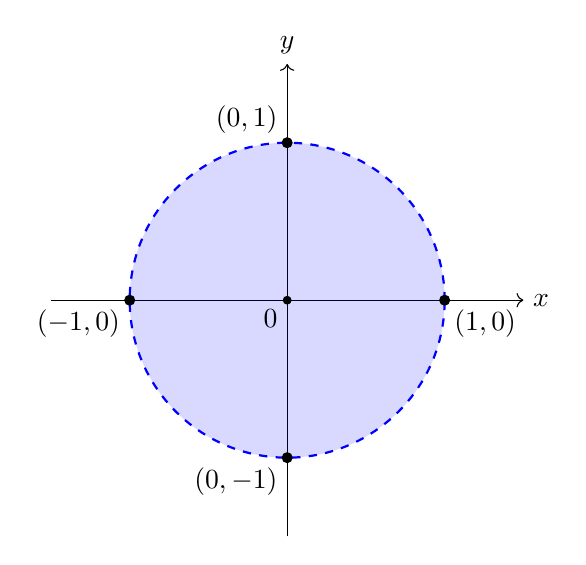
\begin{tikzpicture}[scale=2]

    % Coordinate axes
    \draw[->] (-1.5,0) -- (1.5,0) node[right] {$x$};
    \draw[->] (0,-1.5) -- (0,1.5) node[above] {$y$};

    % Open ball interior
    \fill[blue, fill opacity=0.15] (0,0) circle (1);

    % Open boundary
    \draw[blue, thick, dashed] (0,0) circle (1);

    % Center
    \fill (0,0) circle (0.8pt);
    \node[below left] at (0,0) {$0$};

    % Radius
    \fill (0,1) circle (1pt);
    \node[above left] at (0,1) {$(0,1)$};
    \fill (1,0) circle (1pt);
    \node[below right] at (1,0) {$(1,0)$};
    \fill (0,-1) circle (1pt);
    \node[below left] at (-1,0) {$(-1,0)$};
    \fill (-1,0) circle (1pt);
    \node[below left] at (0,-1) {$(0, -1)$};

\end{tikzpicture}
\end{center}

\noindent
Open ball $B([0,1]^\top,2)$ in the metric $\alpha$. Center of the ball $(0,1)$ is contained in the open ball since $\alpha([0,1]^\top, [0,1]^\top) = 0 < 2$.
The same is true for a center of any open ball.

\begin{center}
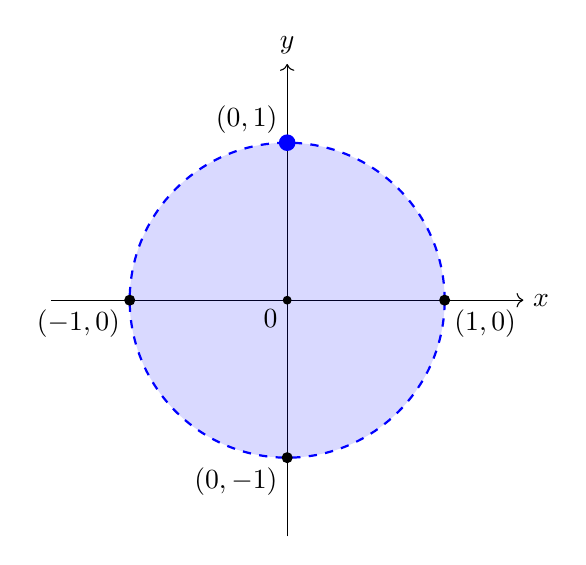
\begin{tikzpicture}[scale=2]

    % Coordinate axes
    \draw[->] (-1.5,0) -- (1.5,0) node[right] {$x$};
    \draw[->] (0,-1.5) -- (0,1.5) node[above] {$y$};

    % Open ball interior
    \fill[blue, fill opacity=0.15] (0,0) circle (1);

    % Open boundary
    \draw[blue, thick, dashed] (0,0) circle (1);

    % Center
    \fill (0,0) circle (0.8pt);
    \node[below left] at (0,0) {$0$};

    % Radius
    \fill[blue] (0,1) circle (1.5pt);
    \node[above left] at (0,1) {$(0,1)$};
    \fill (1,0) circle (1pt);
    \node[below right] at (1,0) {$(1,0)$};
    \fill (0,-1) circle (1pt);
    \node[below left] at (-1,0) {$(-1,0)$};
    \fill (-1,0) circle (1pt);
    \node[below left] at (0,-1) {$(0, -1)$};

\end{tikzpicture}
\end{center}


Open ball $B([1, 2]^\top,1 + \sqrt{5})$ in the metric $\alpha$:

\begin{center}
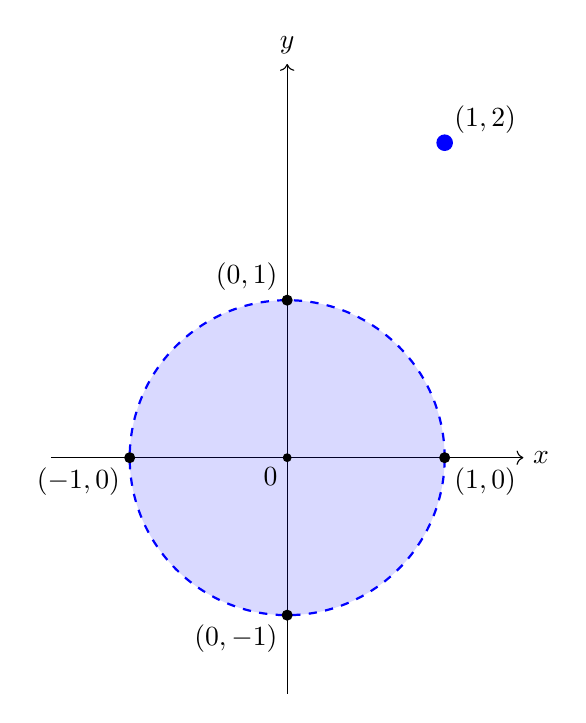
\begin{tikzpicture}[scale=2]

    % Coordinate axes
    \draw[->] (-1.5,0) -- (1.5,0) node[right] {$x$};
    \draw[->] (0,-1.5) -- (0,2.5) node[above] {$y$};

    % Open ball interior
    \fill[blue, fill opacity=0.15] (0,0) circle (1);

    % Open boundary
    \draw[blue, thick, dashed] (0,0) circle (1);

    % Center
    \fill (0,0) circle (0.8pt);
    \node[below left] at (0,0) {$0$};

    % Radius
    \fill (0,1) circle (1pt);
    \node[above left] at (0,1) {$(0,1)$};
    \fill (1,0) circle (1pt);
    \node[below right] at (1,0) {$(1,0)$};
    \fill (0,-1) circle (1pt);
    \node[below left] at (-1,0) {$(-1,0)$};
    \fill (-1,0) circle (1pt);
    \node[below left] at (0,-1) {$(0, -1)$};


        % Point (1,2)
    \fill[blue] (1,2) circle (1.5pt);
    \node[above right] at (1,2) {$(1,2)$};


\end{tikzpicture}
\end{center}

\subsection{Part c)}
Open ball $B(0,1)$ in the metric $\beta$:

\begin{center}
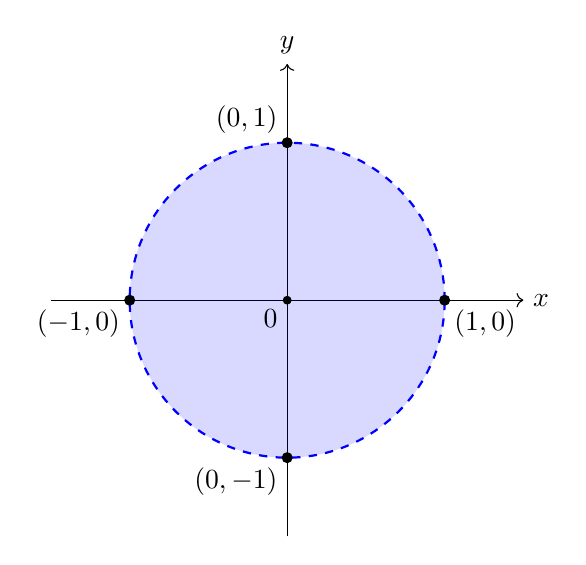
\begin{tikzpicture}[scale=2]

    % Coordinate axes
    \draw[->] (-1.5,0) -- (1.5,0) node[right] {$x$};
    \draw[->] (0,-1.5) -- (0,1.5) node[above] {$y$};

    % Open ball interior
    \fill[blue, fill opacity=0.15] (0,0) circle (1);

    % Open boundary
    \draw[blue, thick, dashed] (0,0) circle (1);

    % Center
    \fill (0,0) circle (0.8pt);
    \node[below left] at (0,0) {$0$};

    % Radius
    \fill (0,1) circle (1pt);
    \node[above left] at (0,1) {$(0,1)$};
    \fill (1,0) circle (1pt);
    \node[below right] at (1,0) {$(1,0)$};
    \fill (0,-1) circle (1pt);
    \node[below left] at (-1,0) {$(-1,0)$};
    \fill (-1,0) circle (1pt);
    \node[below left] at (0,-1) {$(0, -1)$};

\end{tikzpicture}
\end{center}

\noindent
Open ball $B([0,1]^\top,2)$ in the metric $\beta$.

\begin{center}
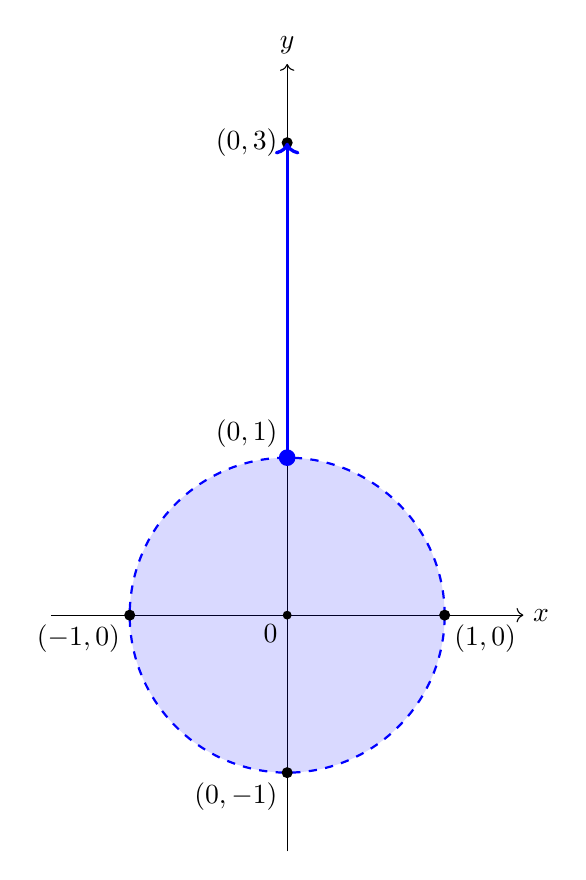
\begin{tikzpicture}[scale=2]

    % Coordinate axes
    \draw[->] (-1.5,0) -- (1.5,0) node[right] {$x$};
    \draw[->] (0,-1.5) -- (0,3.5) node[above] {$y$};

    % Open ball interior
    \fill[blue, fill opacity=0.15] (0,0) circle (1);

    % Open boundary
    \draw[blue, thick, dashed] (0,0) circle (1);

    % Center
    \fill (0,0) circle (0.8pt);
    \node[below left] at (0,0) {$0$};

    % Radius
    \fill[blue] (0,1) circle (1.5pt);
    \node[above left] at (0,1) {$(0,1)$};
    \fill (1,0) circle (1pt);
    \node[below right] at (1,0) {$(1,0)$};
    \fill (0,-1) circle (1pt);
    \node[below left] at (-1,0) {$(-1,0)$};
    \fill (-1,0) circle (1pt);
    \node[below left] at (0,-1) {$(0, -1)$};
    \fill (0,3) circle (1pt);
    \node[left] at (0,3) {$(0, 3)$};

    \draw[blue, very thick, ->] (0,1) -- (0,3);
        

\end{tikzpicture}
\end{center}


Open ball $B([2, 2]^\top, \sqrt{2})$ in the metric $\beta$:

\begin{center}
\begin{tikzpicture}[scale=2]

    % Coordinate axes
    \draw[->] (-1,0) -- (4,0) node[right] {$x$};
    \draw[->] (0,-1) -- (0,4) node[above] {$y$};


    % Center
    \fill (0,0) circle (0.8pt);
    \node[below left] at (0,0) {$0$};

    \fill (1,1) circle (1pt);
    \node[right] at (1,1) {$(1, 1)$};
    \fill (3,3) circle (1pt);
    \node[left] at (3,3) {$(3, 3)$};
    
    \draw[blue, very thick, <->] (1,1) -- (3,3);


\end{tikzpicture}
\end{center}

\noindent
\textbf{Explanation}: Let $y = [y_1 \quad y_2]^\top \in \mathbb{R}^2$. Two cases: 
\begin{itemize}
    \item Assume $x_1y_2 = x_2y_1$. In our case $x_1 = x_2 = 2$, so $2y_2 = 2y_1$ or $y_2 = y_1$. By the definition of
    $\beta$, the open ball $B([2, 2]^\top, \sqrt{2})$ includes points $(y_1, y_1)$ such that $\lVert (2,2) - (y_1, y_1)\rVert < \sqrt{2}$.
    From this condition we get an inequality $\sqrt{2(2-y_1)^2} < \sqrt{2}$, which gives us $\lvert 2 - y_1 \rvert < 1$.
    This gives the open line segment from $(1,1)$ to $(3,3)$.
    \item Assume $x_1y_2 \neq x_2y_1$. By the definition of $\beta$, the open ball $B([2, 2]^\top, \sqrt{2})$ includes points $(y_1, y_2)$ 
    such that $\sqrt{8} + \lVert (y_1, y_2) \rVert < \sqrt{2}$. Since there is no such vector $y$, this gives us an empty set.
\end{itemize}

\subsection{Part d)}

Open ball $B(0,1)$ in the metric $\gamma$:

\begin{center}
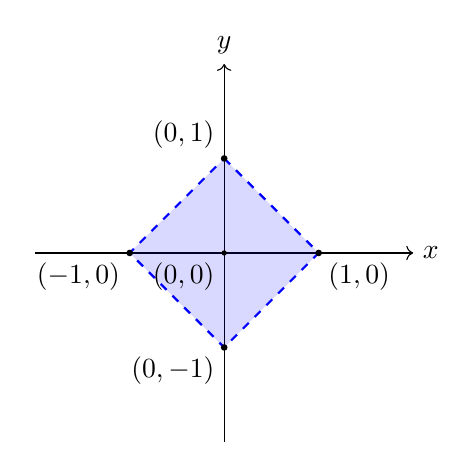
\begin{tikzpicture}[scale=1.2]

    % Coordinate axes
    \draw[->] (-2,0) -- (2,0) node[right] {$x$};
    \draw[->] (0,-2) -- (0,2) node[above] {$y$};

    % Open ball interior
    \fill[blue, fill opacity=0.15]
        (0,1) -- (1,0) -- (0,-1) -- (-1,0) -- cycle;

    % Boundary 
    \draw[blue, thick, dashed]
        (0,1) -- (1,0) -- (0,-1) -- (-1,0) -- cycle;

    % Center
    \fill (0,0) circle (0.8pt);
    \node[below left] at (0,0) {$(0,0)$};

    % Radius
    \fill (0,1) circle (1pt);
    \node[above left] at (0,1) {$(0,1)$};
    \fill (1,0) circle (1pt);
    \node[below right] at (1,0) {$(1,0)$};
    \fill (0,-1) circle (1pt);
    \node[below left] at (-1,0) {$(-1,0)$};
    \fill (-1,0) circle (1pt);
    \node[below left] at (0,-1) {$(0, -1)$};


\end{tikzpicture}
\end{center}

\noindent
Open ball $ B([0,2]^\top,3)$ in the metric $\gamma$:

\begin{center}
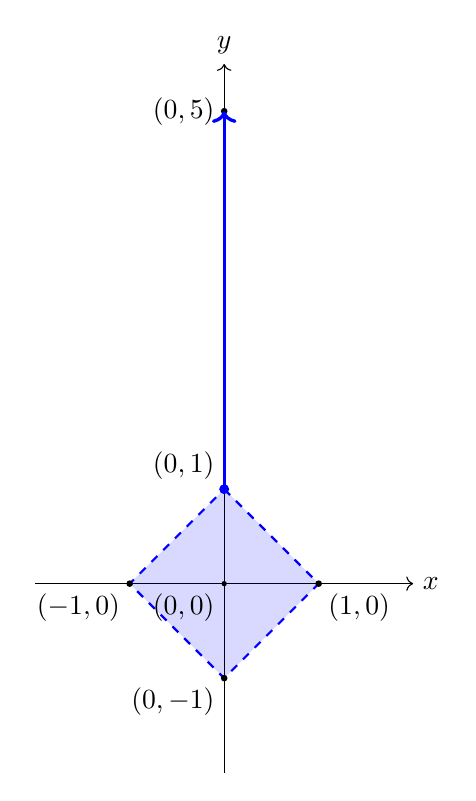
\begin{tikzpicture}[scale=1.2]

    % Coordinate axes
    \draw[->] (-2,0) -- (2,0) node[right] {$x$};
    \draw[->] (0,-2) -- (0,5.5) node[above] {$y$};

    % Open ball interior
    \fill[blue, fill opacity=0.15]
        (0,1) -- (1,0) -- (0,-1) -- (-1,0) -- cycle;

    % Boundary 
    \draw[blue, thick, dashed]
        (0,1) -- (1,0) -- (0,-1) -- (-1,0) -- cycle;

    % Center
    \fill (0,0) circle (0.8pt);
    \node[below left] at (0,0) {$(0,0)$};

    % Radius
    \fill[blue] (0,1) circle (1.5pt);
    \node[above left] at (0,1) {$(0,1)$};
    \fill (1,0) circle (1pt);
    \node[below right] at (1,0) {$(1,0)$};
    \fill (0,-1) circle (1pt);
    \node[below left] at (-1,0) {$(-1,0)$};
    \fill (-1,0) circle (1pt);
    \node[below left] at (0,-1) {$(0, -1)$};
    \fill (0,5) circle (1pt);
    \node[left] at (0,5) {$(0, 5)$};

    \draw[blue, very thick, ->] (0,1) -- (0,5);

\end{tikzpicture}
\end{center}

\noindent
Open ball $ B([1,-1]^\top,2)$ in the metric $\gamma$:


\begin{center}
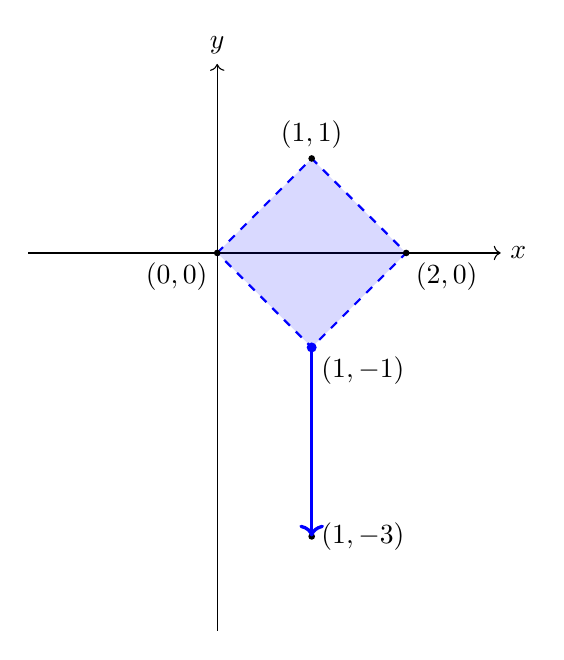
\begin{tikzpicture}[scale=1.2]

    % Coordinate axes
    \draw[->] (-2,0) -- (3,0) node[right] {$x$};
    \draw[->] (0,-4) -- (0,2) node[above] {$y$};

    % Open ball interior
    \fill[blue, fill opacity=0.15]
        (0,0) -- (1,1) -- (2,0) -- (1,-1) -- cycle;

    % Boundary 
    \draw[blue, thick, dashed]
        (0,0) -- (1,1) -- (2,0) -- (1,-1) -- cycle;

    % Center
    \fill (0,0) circle (1pt);
    \node[below left] at (0,0) {$(0,0)$};

    % Radius
    \fill[blue] (1,-1) circle (1.5pt);
    \node[below right] at (1,-1) {$(1,-1)$};
    \fill (2,0) circle (1pt);
    \node[below right] at (2,0) {$(2,0)$};
    \fill (1,1) circle (1pt);
    \node[above] at (1,1) {$(1, 1)$};
    \fill (1,-3) circle (1pt);
    \node[right] at (1,-3) {$(1, -3)$};

    \draw[blue, very thick, ->] (1,-1) -- (1,-3);

\end{tikzpicture}
\end{center}

\section{Problem 2: Homeomorphic spaces}

We are given spaces $X_n = S^{n-1} \times [0,1]$, $Y_n = \{(x_1, \ldots, x_n) \in \mathbb{R}^n; \quad 1 \leq x_1^2 + ... + x_n^2 \leq 4\}$.
Our task is to show these two spaces are homeomorphic for any $n \in \mathbb{N}$. We firstcheck out how these two spaces look like for
$n=1$ and $n=2$.


\pagebreak
\noindent
$X_1$:

\begin{center}
\begin{tikzpicture}[scale=1.5]

% Coordinate axes
\draw[->] (-2,0) -- (2,0) node[right] {$x$};
\draw[->] (0,-0.5) -- (0,1.6) node[above] {$t$};



% Boundaries
\draw[blue, very thick] (-1,0) -- (-1,1);
\draw[blue, very thick] (1,0) -- (1,1);

% Endpoints
\foreach \x in {-1,1}
{
    \fill[blue] (\x,0) circle (1.5pt);
    \fill[blue] (\x,1) circle (1.5pt);
}

% Coordinate labels
\node[below left] at (-1,0) {$(-1,0)$};
\node[below right] at (1,0) {$(1,0)$};

\node[left] at (-1,1) {$(-1,1)$};
\node[right] at (1,1) {$(1,1)$};


\end{tikzpicture}
\end{center}

\vspace{10mm} %5mm vertical space

\noindent
$Y_1$:

\begin{center}
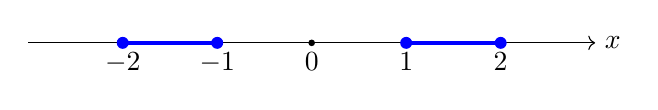
\begin{tikzpicture}[scale=1.2]

% Coordinate axis
\draw[->] (-3,0) -- (3,0) node[right] {$x$};

% Intervals



% Boundaries
\draw[blue, very thick] (-2,0) -- (-1,0);
\draw[blue, very thick] (1,0) -- (2,0);

% Endpoints
\foreach \x in {-2,-1,1,2}
    \fill[blue] (\x,0) circle (1.8pt);

% Labels
\node[below] at (-2,0) {$-2$};
\node[below] at (-1,0) {$-1$};
\node[below] at (1,0) {$1$};
\node[below] at (2,0) {$2$};
\node[below] at (0,0) {$0$};
\fill (0,0) circle (1pt);


\end{tikzpicture}
\end{center}

\noindent
We want to show $X_1 \cong Y_1$. We define a map $f: X_1 \rightarrow Y_1$ as 
\begin{equation*}
  f(x,t) =
    \begin{cases}
      t-2; & \quad x < 0\\
      t+1; &\quad x \geq 0.
    \end{cases}       
\end{equation*}

\noindent
This is a peicewise continuous map with a peicewise continuous inverse

\begin{equation*}
  f^{-1}(x) =
    \begin{cases}
      (-1, x+2); &\quad x < 0\\
      (1, x-1); &\quad x \geq 0,
    \end{cases}       
\end{equation*}

\noindent
so $f$ is a homeomorphism. 

\vspace{10mm} %5mm vertical space
\noindent
$X_2$:

\begin{center}
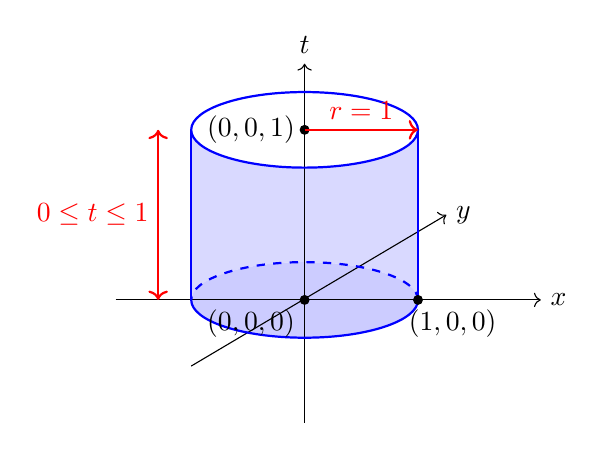
\begin{tikzpicture}[scale=1.2]


% Cylinder dimensions
\def\rx{1.2}
\def\ry{0.4}
\def\h{1.8}

% Shaded lateral surface
\fill[blue, fill opacity=0.15]
    (-\rx,0) --
    (-\rx,\h)
    arc[start angle=180,end angle=360,
        x radius={\rx},y radius={\ry}]
    -- (\rx,0)
    arc[start angle=0,end angle=180,
        x radius={\rx},y radius={\ry}]
    -- cycle;

 % Shaded bottom disk
\fill[blue!20] (0,0) ellipse ({\rx} and {\ry});

% Top and bottom disks are NOT filled:
% only the circular boundary curves belong to X_2.

% Coordinate axes
\draw[->] (-2,0) -- (2.5,0) node[right] {$x$};
\draw[->] (-1.2,-0.7) -- (1.5,0.9) node[right] {$y$};
\draw[->] (0,-1.3) -- (0,2.5) node[above] {$t$};

% Vertical boundary curves
\draw[blue, thick] (-\rx,0) -- (-\rx,\h);
\draw[blue, thick] (\rx,0) -- (\rx,\h);

% Top circle
\draw[blue, thick]
    (0,\h) ellipse ({\rx} and {\ry});

% Bottom circle
\draw[blue, thick]
    (-\rx,0)
    arc[start angle=180,end angle=360,
        x radius={\rx},y radius={\ry}];

\draw[blue, thick, dashed]
    (\rx,0)
    arc[start angle=0,end angle=180,
        x radius={\rx},y radius={\ry}];

% Top and bottom center points
\fill (0,0) circle (1.5pt);
\fill (0,\h) circle (1.5pt);
\fill (1.2,0) circle (1.5pt);

\node[below left] at (0,0) {$(0,0,0)$};
\node[left] at (0,\h) {$(0,0,1)$};
\node[below right] at (1,0) {$(1,0,0)$};

% Radius on top circle
\draw[red, thick, ->]
    (0,\h) -- (\rx,\h)
    node[midway,above] {$r=1$};

% Height
\draw[red, thick, <->]
    (-1.55,0) -- (-1.55,\h);

\node[left,red] at (-1.55,0.9) {$0\leq t\leq1$};


\end{tikzpicture}
\end{center}


\pagebreak
\noindent
$Y_2$:

\begin{center}
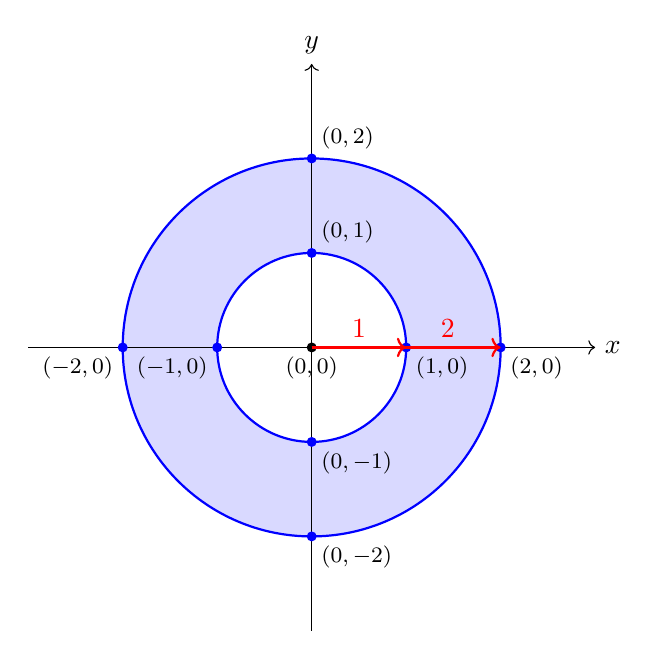
\begin{tikzpicture}[scale=1.2]

% Shaded annulus
\fill[blue, fill opacity=0.15]
    (0,0) circle (2);

\fill[white]
    (0,0) circle (1);

% Coordinate axes
\draw[->] (-3,0) -- (3,0) node[right] {$x$};
\draw[->] (0,-3) -- (0,3) node[above] {$y$};

% Boundaries
\draw[blue, thick] (0,0) circle (2);
\draw[blue, thick] (0,0) circle (1);

% Center
\fill (0,0) circle (1.5pt);
\node[below, font=\footnotesize] at (0,0) {$(0,0)$};

% Outer circle points
\foreach \x/\y/\pos in {
    2/0/below right,
    -2/0/below left,
    0/2/above right,
    0/-2/below right}
{
    \fill[blue] (\x,\y) circle (1.5pt);
    \node[\pos, font=\footnotesize] at (\x,\y) {$ (\x,\y) $};
}

% Inner circle points
\fill[blue] (1,0) circle (1.5pt);
\node[below right, font=\footnotesize] at (1,0) {$(1,0)$};

\fill[blue] (-1,0) circle (1.5pt);
\node[below left, font=\footnotesize] at (-1,0) {$(-1,0)$};

\fill[blue] (0,1) circle (1.5pt);
\node[above right, font=\footnotesize] at (0,1) {$(0,1)$};

\fill[blue] (0,-1) circle (1.5pt);
\node[below right, font=\footnotesize] at (0,-1) {$(0,-1)$};

% Radii
\draw[red, thick, ->] (0,0) -- (1,0)
    node[midway,above] {$1$};

\draw[red, thick, ->] (0,0) -- (2,0)
    node[midway,above, xshift=15pt] {$2$};



\end{tikzpicture}
\end{center}

\noindent
Similarly to $n=1$ case, we can define a map $f: X_2 \rightarrow Y_2$ as

\begin{equation*}
  f(x,y,t) = (x(1+t), y(1+t))
\end{equation*}

\noindent
This is a continuous map with a continuous inverse

\begin{equation*}
  f^{-1}(x, y) = \Big(\frac{(x,y)}{\lVert (x,y)\rVert}, \lVert (x,y)\rVert - 1 \Big),
\end{equation*}

\noindent
so $f$ is a homeomorphism. For a general case, we construct a map $f: X_n \rightarrow Y_n$ as

\begin{equation*}
  f(u, t) = (1+t)u, \quad u \in S^{n-1}, \; t \in [0,1].  
\end{equation*}

\noindent
This map is a homeomorphism since it is continuous and has a continuous inverse. From this we conclude 
$\forall n \in \mathbb{N}$, $X_n \cong Y_n$.

\section{Problem 3: Chessboard complex}

\subsection{Part a)}
We want to show that chessboard complex $\Delta_{3 \times 2}$ is homeomorphic to the circle $S^1$. The complex looks like this:

% Figure 1: The 2 x 3 chessboard
\begin{figure}[h]
\centering
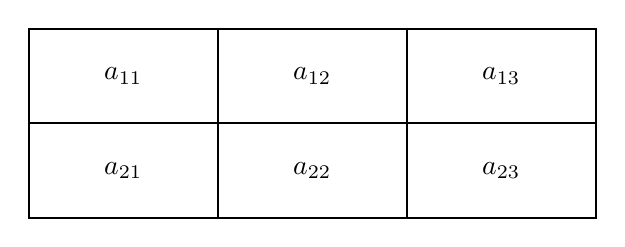
\begin{tikzpicture}[scale=1.2]

    % Draw the chessboard
    \draw[thick] (0,0) rectangle (6,2);
    \draw[thick] (2,0) -- (2,2);
    \draw[thick] (4,0) -- (4,2);
    \draw[thick] (0,1) -- (6,1);

    % Labels inside the squares
    \node at (1,1.5) {$a_{11}$};
    \node at (3,1.5) {$a_{12}$};
    \node at (5,1.5) {$a_{13}$};

    \node at (1,0.5) {$a_{21}$};
    \node at (3,0.5) {$a_{22}$};
    \node at (5,0.5) {$a_{23}$};

\end{tikzpicture}
\caption{The $2\times3$ chessboard.}
\end{figure}


% Figure 2: The chessboard complex
\begin{figure}[h]
\centering
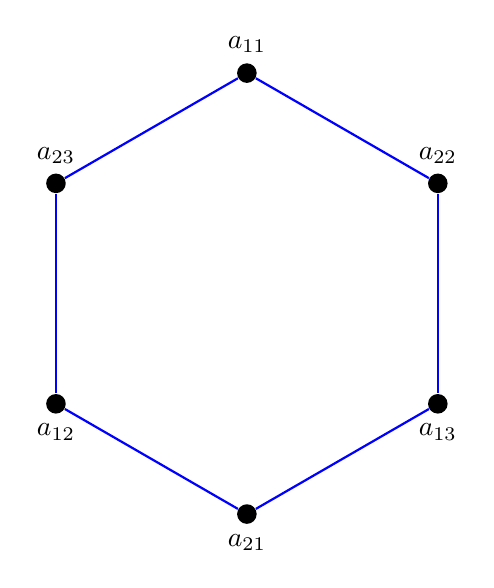
\begin{tikzpicture}[scale=1.4,
    vertex/.style={circle, fill=black, inner sep=2.5pt},
    edge/.style={thick, blue}]

    % Vertices
    \node[vertex,label=above:$a_{11}$] (v1) at (90:2) {};
    \node[vertex,label=above:$a_{22}$] (v2) at (30:2) {};
    \node[vertex,label=below:$a_{13}$] (v3) at (-30:2) {};
    \node[vertex,label=below:$a_{21}$] (v4) at (-90:2) {};
    \node[vertex,label=below:$a_{12}$] (v5) at (-150:2) {};
    \node[vertex,label=above:$a_{23}$] (v6) at (150:2) {};

    % Edges
    \draw[edge] (v1) -- (v2);
    \draw[edge] (v2) -- (v3);
    \draw[edge] (v3) -- (v4);
    \draw[edge] (v4) -- (v5);
    \draw[edge] (v5) -- (v6);
    \draw[edge] (v6) -- (v1);

\end{tikzpicture}
\caption{The chessboard complex $\Delta_{2\times3}$.}
\label{fig:delta32}
\end{figure}

\noindent
The edges represent exactly the six possible pairs of non-attacking rooks:
\[
\begin{aligned}
E=\{&
\{a_{11},a_{22}\},
\{a_{11},a_{23}\},\\
&\{a_{12},a_{21}\},
\{a_{12},a_{23}\},\\
&\{a_{13},a_{21}\},
\{a_{13},a_{22}\}
\}.
\end{aligned}
\]

\noindent
We cannot place 3 non-attacking rooks on the $3 \times 2$ chessboard, therefore there are no triangles (2-simplices) in
$\Delta_{2\times3}$. It follows that $\Delta_{2\times3}$ is a 1-dimensional simplicial complex. To prove connectivity of a simplicial complex, we
need to show that its 1-skeleton (the graph consisting of its vertices and edges) is connected. This is obvious from figure \ref{fig:delta32}.
It also holds that every vertex has degree 2. From these observations, we can conclude that $\Delta_{2\times3}$ is a cycle $C_6$.
It follows that $\Delta_{2\times3}$ is homeomorphic to a circle $S^1$.

\subsection{Part b)}
We want to show that chessboard complex $\Delta_{4 \times 3}$ is homeomorphic to a torus $S^1 \times S^1$. 

\begin{figure}[h]
\centering
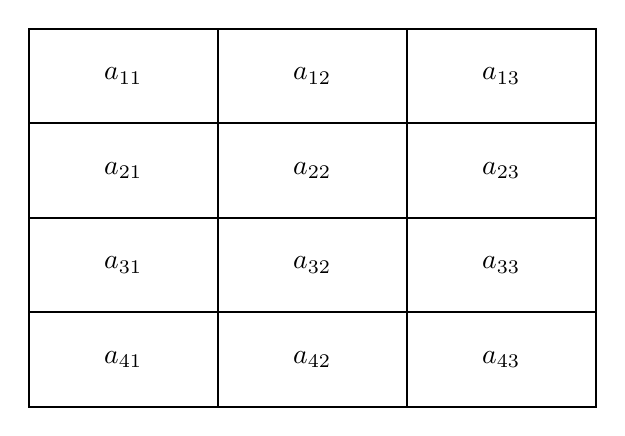
\begin{tikzpicture}[scale=1.2]

    % Draw the chessboard
    \draw[thick] (0,0) rectangle (6,4);
    \draw[thick] (2,0) -- (2,4);
    \draw[thick] (4,0) -- (4,4);
    \draw[thick] (0,1) -- (6,1);
    \draw[thick] (0,2) -- (6,2);
    \draw[thick] (0,3) -- (6,3);

    % Labels inside the squares
    \node at (1,3.5) {$a_{11}$};
    \node at (3,3.5) {$a_{12}$};
    \node at (5,3.5) {$a_{13}$};

    \node at (1,2.5) {$a_{21}$};
    \node at (3,2.5) {$a_{22}$};
    \node at (5,2.5) {$a_{23}$};

    \node at (1,1.5) {$a_{31}$};
    \node at (3,1.5) {$a_{32}$};
    \node at (5,1.5) {$a_{33}$};

    \node at (1,0.5) {$a_{41}$};
    \node at (3,0.5) {$a_{42}$};
    \node at (5,0.5) {$a_{43}$};

\end{tikzpicture}
\caption{The $4\times3$ chessboard.}
\end{figure}


\begin{figure}[h]
\centering
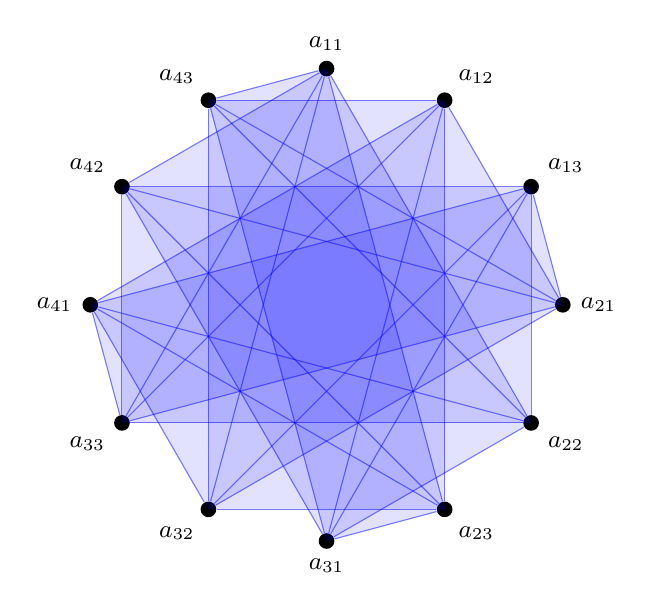
\begin{tikzpicture}[scale=1.5,
    vertex/.style={circle, fill=black, inner sep=2pt},
    edge/.style={thin, blue, opacity=0.5},
    face/.style={fill=blue, opacity=0.06, draw=none}]

    % Vertices: 12 points on a circle, ordered a_11, a_12, a_13, a_21, ...
    \foreach \i in {1,...,4} {
        \foreach \j in {1,2,3} {
            \pgfmathtruncatemacro{\k}{3*(\i-1)+\j-1}
            \pgfmathsetmacro{\ang}{90-30*\k}
            \node[vertex, label={[font=\small]\ang:$a_{\i\j}$}] (v\i\j) at (\ang:2) {};
        }
    }

    % Triangles: one rook in each column, in three distinct rows
    \foreach \p in {1,...,4} {
        \foreach \q in {1,...,4} {
            \foreach \s in {1,...,4} {
                \ifnum\p=\q\else
                \ifnum\q=\s\else
                \ifnum\p=\s\else
                    \fill[face] (v\p1.center) -- (v\q2.center) -- (v\s3.center) -- cycle;
                \fi\fi\fi
            }
        }
    }

    % Edges: a_{ij} -- a_{kl} whenever i != k and j != l
    \foreach \i in {1,...,4} {
        \foreach \j in {1,2,3} {
            \foreach \k in {1,...,4} {
                \foreach \l in {1,2,3} {
                    \ifnum\i<\k\relax
                        \ifnum\j=\l\relax\else
                            \draw[edge] (v\i\j) -- (v\k\l);
                        \fi
                    \fi
                }
            }
        }
    }
\end{tikzpicture}
\caption{The chessboard complex $\Delta_{4\times3}$.}
\label{fig:delta43}
\end{figure}

\noindent
The complex $\Delta_{4\times3}$ has 12 vertices:
$$V = \{a_{ij}; \; 1 \leq i \leq 4, \; 1 \leq j \leq 3 \},$$

\noindent
$\binom{4}{2} \cdot 3 \cdot 2 = 36$ edges:
$$E = \{ \{a_{ij}, a_{kl}\}; \; 1 \leq i \leq 4, \; 1 \leq j \leq 3, \; i \neq k, \; j \neq l \},$$

\noindent
and $\binom{4}{3} \cdot 3! = 24$ triangles. It has no simplices of dimension $\geq$ 3, since we cant put 4 non-attacking rooks
on a $4 \times 3$ chessboard. This means $\Delta_{4 \times 3}$ is a 2-dimensional manifold. It is obvious from figure \ref{fig:delta43}
that it is connected. We can compute its Euler characteristic:
$$\chi = V - E + F = 12 - 36 + 24 = 0.$$ 

\noindent
Let us compute the boundary of $\Delta_{4 \times 3}$. Since it is a 2-dimensional complex, its boundary would be a set of edges.
An edge is a boundary edge if it belongs to exactly one triangle (otherwise the edge cancels out with an edge of a second trinagle, if they are
consistently oriented). In our case, there is no such edge because for every pair
$\{a_{ij}, a_{kl}\}$, there are exactly 2 vertices $a_{pq}$ satisfying $p \neq i,k, \; q \neq j,l$. This is because there are exactly two rows different from \(i\) and \(k\), since we have four rows,
and there is exactly one column different from \(j\) and \(l\), since we have three columns.
To prove $\Delta_{4 \times 3} \cong S^1 \times S^1$, we need to show that $\Delta_{4 \times 3}$ is orientable: there exists a consistent orientation of its $2$-simplices.

\noindent
Every triangle has one rook in each column, so it has a canonical ordering $T(a,b,c) = [(a,1),(b,2),(c,3)]$. 
Let $d$ be the missing row, so $(a,b,c,d)$ is a permutation of ${1,2,3,4}$. We orient each triangle by $\epsilon \cdot T(a,b,c)$ where $\epsilon = \text{sgn}(a,b,c,d)$.
This means that even permutations keep the canonical orientation, and odd ones reverse it.
Two triangles share an edge exactly when they agree in two columns and differ in the third. Each edge lies in exactly two triangles:

\vspace*{10px}

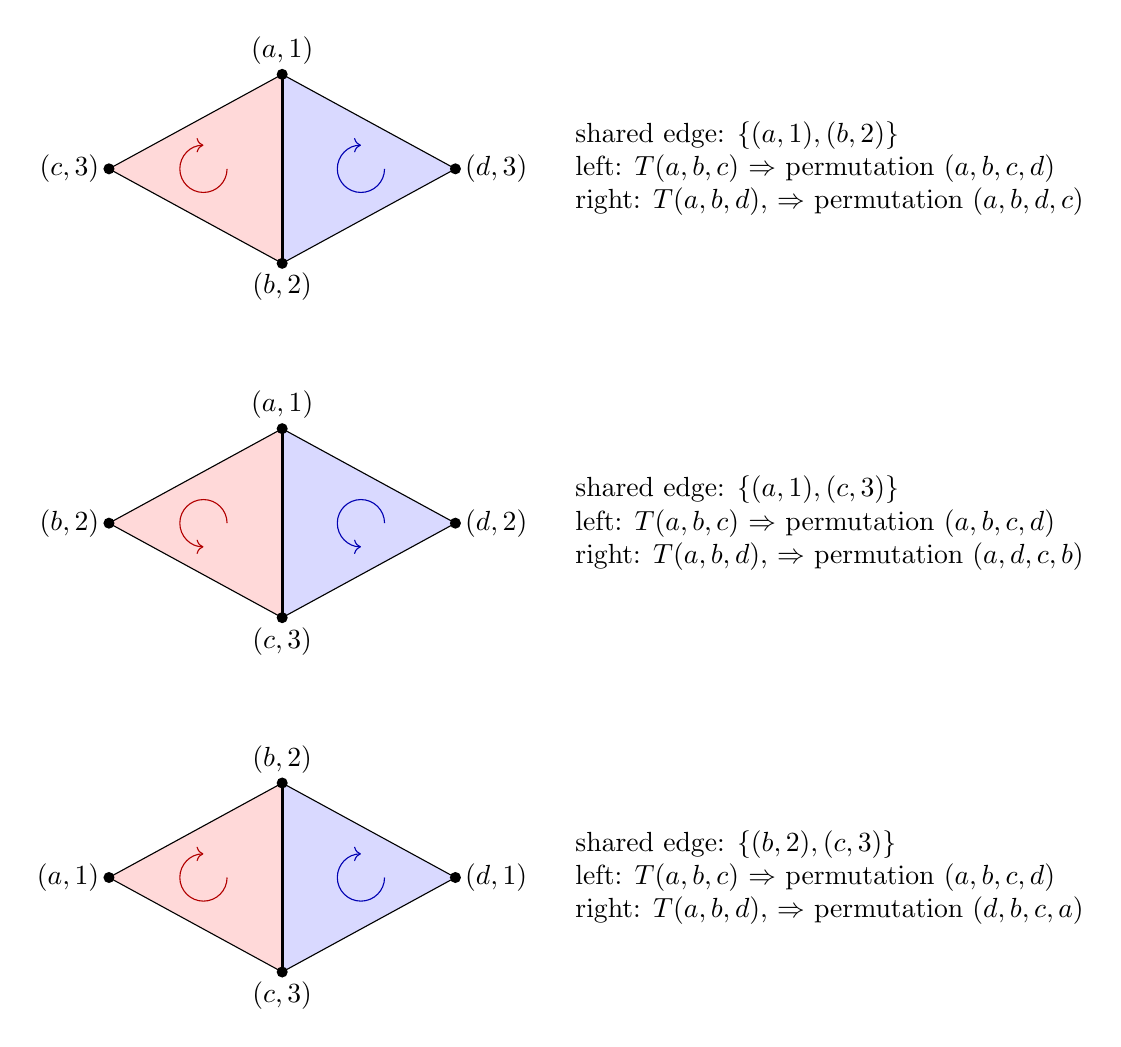
\begin{tikzpicture}

\pair{0}{0}{$(a,1)$}{$(b,2)$}{$(c,3)$}{$(d,3)$}{-270}{-270}
{shared edge: $\{(a,1), (b,2)\}$\\
 left: $T(a,b,c)$ $\Rightarrow$ permutation $(a,b,c,d)$\\
 right: $T(a,b,d)$, $\Rightarrow$ permutation $(a,b,d,c)$}

\pair{0}{-4.5}{$(a,1)$}{$(c,3)$}{$(b,2)$}{$(d,2)$}{270}{270}
{shared edge: $\{(a,1), (c,3)\}$\\
 left: $T(a,b,c)$ $\Rightarrow$ permutation $(a,b,c,d)$\\
 right: $T(a,b,d)$, $\Rightarrow$ permutation $(a,d,c,b)$}

\pair{0}{-9}{$(b,2)$}{$(c,3)$}{$(a,1)$}{$(d,1)$}{-270}{-270}
{shared edge: $\{(b,2), (c,3)\}$\\
 left: $T(a,b,c)$ $\Rightarrow$ permutation $(a,b,c,d)$\\
 right: $T(a,b,d)$, $\Rightarrow$ permutation $(d,b,c,a)$}

\end{tikzpicture}

\noindent
Each pair of permutations differ by a transposition, so $\epsilon$ is opposite on the two triangles. This is true for any given triangle in $\Delta_{4 \times 3}$. It follows that that each pair of triangles
is consistently oriented. With this, we can conclude that $\Delta_{4 \times 3}$ is orientable. \\

\noindent
We have shown that $\Delta_{4 \times 3}$  is an orientable connected 2-dimensional manifold without boundary with Euler characteristic 0.
By the Classification theorem, it follows that $\Delta_{4 \times 3} \cong S^1 \times S^1$.


\subsection{Part c)}

Our task is to find out whether the chessboard complex $\Delta_{n \times (n-1)}$ is a manifold for all $n \in \N$.
To do that, first draw the link of an arbirtaty vertex of $\Delta_{n \times (n-1)}$. Reminder: For a simplicial complex $K$ and simplex $\sigma \in K$,
a \textbf{link} of $\sigma$ is
$$\text{Lk}(\sigma) = \{\tau \in K; \; \tau \cap \sigma = \varnothing, \; \tau \cup \sigma \in K\} \leq K.$$

\tikzset{
  v/.style={circle,draw,inner sep=1pt,minimum size=15pt,font=\scriptsize},
  every edge/.style={draw,thick}
}

%% ---------- (1) link of a vertex in Delta_{3,2} : two points ----------
\begin{figure}[H]
\centering
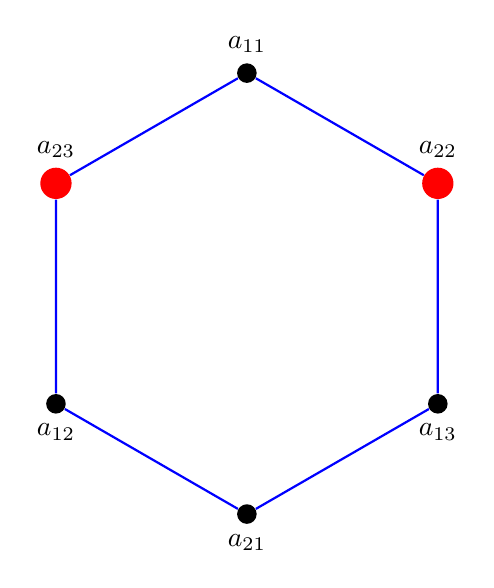
\begin{tikzpicture}[scale=1.4,
    vertex/.style={circle, fill=black, inner sep=2.5pt},
    highlight/.style={circle, fill=red, inner sep=4pt},
    edge/.style={thick, blue}]

% Vertices
\node[vertex,label=above:$a_{11}$] (v1) at (90:2) {};
\node[highlight,label=above:$a_{22}$] (v2) at (30:2) {};
\node[vertex,label=below:$a_{13}$] (v3) at (-30:2) {};
\node[vertex,label=below:$a_{21}$] (v4) at (-90:2) {};
\node[vertex,label=below:$a_{12}$] (v5) at (-150:2) {};
\node[highlight,label=above:$a_{23}$] (v6) at (150:2) {};

% Edges
\draw[edge] (v1) -- (v2);
\draw[edge] (v2) -- (v3);
\draw[edge] (v3) -- (v4);
\draw[edge] (v4) -- (v5);
\draw[edge] (v5) -- (v6);
\draw[edge] (v6) -- (v1);

\end{tikzpicture}
\caption{Link of vertex $a_{11}$ in $\Delta_{3\times 2}$.}
\label{fig:link32}
\end{figure}

\noindent
Notice that the link of any vertex in $\Delta_{3\times 2}$ is homeomorphic to $S^0$.

\vspace*{10px}

\begin{figure}[H]
\centering
\begin{minipage}{0.58\textwidth}
\centering
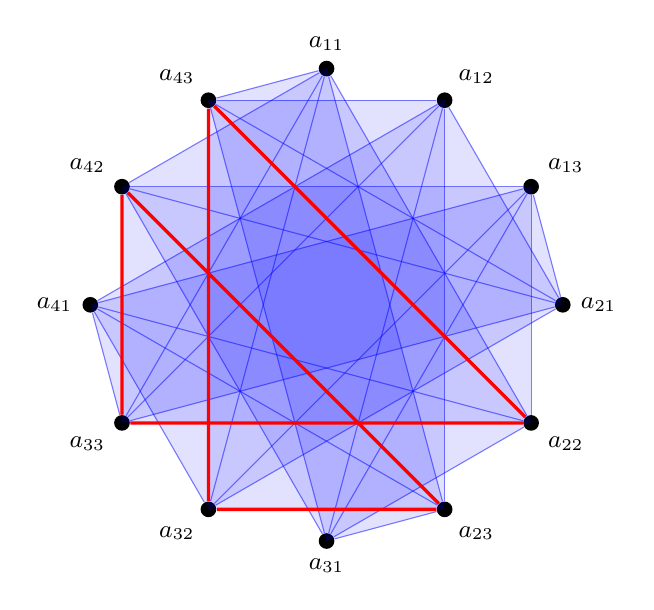
\begin{tikzpicture}[scale=1.5,
    vertex/.style={circle, fill=black, inner sep=2pt},
    edge/.style={thin, blue, opacity=0.5},
    linkedge/.style={very thick, red},
    face/.style={fill=blue, opacity=0.06, draw=none}]

    % Vertices: 12 points on a circle, ordered a_11, a_12, a_13, a_21, ...
    \foreach \i in {1,...,4} {
        \foreach \j in {1,2,3} {
            \pgfmathtruncatemacro{\k}{3*(\i-1)+\j-1}
            \pgfmathsetmacro{\ang}{90-30*\k}
            \node[vertex, label={[font=\small]\ang:$a_{\i\j}$}] (v\i\j) at (\ang:2) {};
        }
    }

    % Triangles: one rook in each column, in three distinct rows
    \foreach \p in {1,...,4} {
        \foreach \q in {1,...,4} {
            \foreach \s in {1,...,4} {
                \ifnum\p=\q\else
                \ifnum\q=\s\else
                \ifnum\p=\s\else
                    \fill[face] (v\p1.center) -- (v\q2.center) -- (v\s3.center) -- cycle;
                \fi\fi\fi
            }
        }
    }

    % Edges: a_{ij} -- a_{kl} whenever i != k and j != l
    \foreach \i in {1,...,4} {
        \foreach \j in {1,2,3} {
            \foreach \k in {1,...,4} {
                \foreach \l in {1,2,3} {
                    \ifnum\i<\k\relax
                        \ifnum\j=\l\relax\else
                            \draw[edge] (v\i\j) -- (v\k\l);
                        \fi
                    \fi
                }
            }
        }
    }

    % Link of a_11: hexagon 22 - 33 - 42 - 23 - 32 - 43 - 22
    \draw[linkedge] (v22) -- (v33) -- (v42) -- (v23) -- (v32) -- (v43) -- (v22);
\end{tikzpicture}
\end{minipage}%
\hfill
\begin{minipage}{0.38\textwidth}
\centering
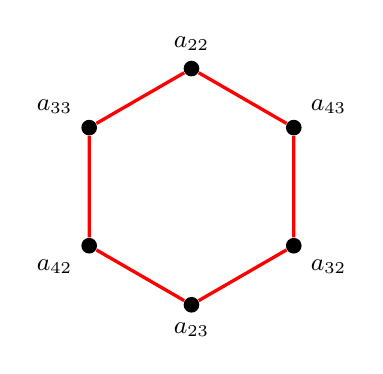
\begin{tikzpicture}[scale=1.5,
    vertex/.style={circle, fill=black, inner sep=2pt},
    linkedge/.style={very thick, red}]

    \foreach \i/\l in {0/22, 1/33, 2/42, 3/23, 4/32, 5/43}{
        \node[vertex, label={[font=\small]{90+60*\i}:$a_{\l}$}] (h\i) at ({90+60*\i}:1) {};
    }
    \foreach \i/\j in {0/1,1/2,2/3,3/4,4/5,5/0}{
        \draw[linkedge] (h\i) -- (h\j);
    }
\end{tikzpicture}
\end{minipage}
\caption{Link of vertex $a_{11}$ in $\Delta_{4\times3}$.}
\label{fig:link43}
\end{figure}


\noindent
Notice that the link of any vertex in $\Delta_{4\times 3}$ is homeomorphic to $S^1$. \\
\noindent
These two examples give us an idea for a general case.

\begin{lemma}
    Let $\Delta_{n \times (n-1)}$ be the chessboard complex from above and let $a_{ij}$ be a vertex in $\Delta_{n \times (n-1)}$.
    Then
    $$\mathrm{Lk}(a_{ij}) = \Delta_{(n-1) \times (n-2)}.$$
\end{lemma}

\begin{proof}
    Take an arbitrary vertex $a_{\tilde{i} \tilde{j}}$ to be a rook (the same as placing a rook on square $(\tilde{i},\tilde{j})$). 
    A set of rooks $R$ make up a simplex in $\text{Lk}(a_{\tilde{i}\tilde{j}})$ when no rook in $R$ is in row $\tilde{i}$ or column $\tilde{j}$
    and none of the rooks in $R$ are attacking each other. This is the same as taking a chessboard, deleting row $\tilde{i}$ and column $\tilde{j}$
    and making another chessboard complex of non-attacking rooks. In other words, $\mathrm{Lk}(a_{ij}) = \Delta_{(n-1) \times (n-2)}$.
\end{proof}


\noindent
Recall from lectures the definition of a combinatorial $n$-manifold.

\begin{definition}
    Let $K$ be a simplicial complex and $n \in \N$. We say that $K$ is a \textbf{combinatorial $n$-manifold} if for each 
    vertex $v \in K$, $\mathrm{Lk}(v)$ is homeomorphic to either $S^{n-1}$ (if $v$ is an interior point) or $B^{n-1}$ (if $v$ is a boundary point).
\end{definition}


\noindent
Using our lemma, we get that $\mathrm{Lk}(\Delta_{5 \times 4}) \cong S^1 \times S^1$, so the link of $\Delta_{5 \times 4}$ is not homeomorphic
to $S^{n-1}$ or or $B^{n-1}$ for any $n$. This means that $\Delta_{5 \times 4}$ is not a manifold. I can assume that for $n > 4$, $\Delta_{n \times (n-1)}$ is not a manifold, but I don't have a way of proving it.

\section{Problem 4: Deciding connectivity}

\section{Problem 5}

\end{document}